\documentclass[12pt,a4paper,oneside]{article}
\usepackage[utf8]{inputenc}
\usepackage[portuguese]{babel}
\usepackage[T1]{fontenc}
\usepackage{times}
\usepackage[left=3cm,right=2cm,top=3cm,bottom=2cm]{geometry}
\usepackage{setspace}
\usepackage{indentfirst}
\usepackage{graphicx}
\usepackage{float}
\usepackage{amsmath}
\usepackage{amsfonts}
\usepackage{amssymb}
\usepackage{booktabs}
\usepackage{multirow}
\usepackage{array}
\usepackage{longtable}
\usepackage{url}
\usepackage[hidelinks]{hyperref}
\usepackage{caption}
\usepackage{subcaption}
\usepackage{listings}
\usepackage{xcolor}

% Configurações ABNT
\onehalfspacing
\setlength{\parindent}{1.25cm}
\setlength{\parskip}{0pt}

% Configuração de títulos
\usepackage{titlesec}
\titleformat{\section}{\normalfont\fontsize{12}{15}\bfseries\uppercase}{\thesection}{1em}{}
\titleformat{\subsection}{\normalfont\fontsize{12}{15}\bfseries}{\thesubsection}{1em}{}
\titleformat{\subsubsection}{\normalfont\fontsize{12}{15}\bfseries}{\thesubsubsection}{1em}{}

% Configuração para código
\lstset{
    basicstyle=\ttfamily\footnotesize,
    breaklines=true,
    frame=single,
    language=Python,
    showstringspaces=false,
    commentstyle=\color{gray},
    keywordstyle=\color{blue},
    stringstyle=\color{red}
}

\begin{document}

% CAPA
\begin{titlepage}
\centering
\vspace*{1cm}

{\fontsize{14}{16}\selectfont\bfseries\uppercase{Universidade do Estado do Amazonas}}\\
{\fontsize{14}{16}\selectfont\bfseries\uppercase{Escola Superior de Tecnologia}}\\
{\fontsize{14}{16}\selectfont\bfseries\uppercase{Curso de Engenharia de Computação}}\\

\vspace{3cm}

{\fontsize{14}{16}\selectfont\bfseries\uppercase{Estudo Comparativo de Algoritmos de Criptografia e Desenvolvimento de Aplicação de Assinatura Digital}}

\vspace{3cm}

{\fontsize{12}{14}\selectfont
\textbf{Autores:}\\
Carlos Lavor Neto\\
Eric Dias Perin\\
Alexandro Pantoja\\
}

\vspace{2cm}

{\fontsize{12}{14}\selectfont
Trabalho apresentado à disciplina de Tópicos Especiais em Computação IV como requisito parcial para avaliação acadêmica.

\vspace{0.5cm}
\textbf{Repositório do Projeto:}\\
\url{https://github.com/CarlosLNeto/crypto-performance-study.git}
}

\vfill

{\fontsize{12}{14}\selectfont
Manaus -- AM\\
2025
}

\end{titlepage}

% RESUMO
\newpage
\section*{RESUMO}

Este trabalho apresenta um estudo abrangente sobre criptografia aplicada, dividido em duas partes complementares. A primeira parte consiste em uma análise comparativa de desempenho computacional entre três algoritmos de criptografia simétrica: Advanced Encryption Standard (AES), Blowfish e Twofish, avaliando métricas de CPU, memória, tempo de execução e throughput. A segunda parte desenvolve uma aplicação prática de envio de mensagens com assinatura digital, implementando geração de certificados ad-hoc e verificação de autenticidade. A metodologia empregada utilizou benchmarks automatizados em Python, com medições precisas de recursos computacionais e análises estatísticas rigorosas. Os resultados da primeira parte demonstram que o AES oferece o melhor throughput médio (277,80 MB/s), enquanto o Blowfish apresenta menor consumo de recursos. Na segunda parte, a aplicação de assinatura digital demonstrou eficácia na garantia de autenticidade, integridade e não-repúdio das mensagens, com tempos de resposta adequados para uso prático. O trabalho contribui para o entendimento prático da criptografia moderna, fornecendo dados quantitativos para seleção de algoritmos e uma implementação funcional de infraestrutura de chave pública.

\vspace{0.5cm}
\noindent\textbf{Palavras-chave:} Criptografia. Algoritmos simétricos. Assinatura digital. Certificados digitais. Desempenho computacional. Segurança da informação.

% SUMÁRIO
\newpage
\tableofcontents

% INTRODUÇÃO
\newpage
\section{INTRODUÇÃO}

A criptografia constitui um dos pilares fundamentais da segurança da informação moderna, desempenhando papel crucial na proteção de dados em diversas aplicações, desde comunicações pessoais até sistemas corporativos críticos e transações financeiras. Com o crescimento exponencial do volume de dados processados diariamente e a necessidade de proteção em tempo real, tanto a escolha adequada de algoritmos criptográficos quanto a implementação de sistemas de autenticação tornaram-se decisões estratégicas que impactam diretamente na performance, segurança e confiabilidade dos sistemas.

Este trabalho aborda duas dimensões complementares da criptografia aplicada: a análise comparativa de algoritmos de criptografia simétrica e o desenvolvimento de uma aplicação prática de assinatura digital. A primeira dimensão foca na avaliação quantitativa de performance dos algoritmos AES (Advanced Encryption Standard), Blowfish e Twofish, enquanto a segunda explora a implementação de mecanismos de autenticação e integridade através de assinaturas digitais com certificados gerados ad-hoc.

A relevância deste estudo reside na necessidade crescente de compreender não apenas os aspectos teóricos da criptografia, mas também suas implicações práticas em termos de performance computacional e implementação de sistemas seguros. A escolha inadequada de algoritmos pode resultar em degradação significativa da performance, consumo excessivo de recursos ou vulnerabilidades de segurança, enquanto a ausência de mecanismos adequados de autenticação pode comprometer a confiabilidade das comunicações.

\subsection{Objetivos}

\subsubsection{Objetivo Geral}

Realizar um estudo abrangente sobre criptografia aplicada, comparando o desempenho computacional de algoritmos simétricos e desenvolvendo uma aplicação funcional de assinatura digital com certificados ad-hoc.

\subsubsection{Objetivos Específicos}

\begin{enumerate}
    \item Implementar benchmarks automatizados para medição precisa de performance dos algoritmos AES, Blowfish e Twofish;
    \item Analisar o comportamento dos algoritmos com diferentes tamanhos de dados e configurações de chave;
    \item Desenvolver uma aplicação de envio de mensagens com assinatura digital;
    \item Implementar geração de certificados digitais ad-hoc para remetente e destinatário;
    \item Realizar análises estatísticas para validar a significância das diferenças observadas;
    \item Avaliar a performance das operações criptográficas de assinatura e verificação;
    \item Gerar visualizações gráficas para facilitar a interpretação dos resultados;
    \item Fornecer recomendações práticas baseadas nos resultados obtidos.
\end{enumerate}

% REFERENCIAL TEÓRICO
\section{REFERENCIAL TEÓRICO}

\subsection{Criptografia Simétrica}

A criptografia simétrica, também conhecida como criptografia de chave secreta, utiliza a mesma chave para as operações de criptografia e descriptografia. Esta abordagem oferece alta eficiência computacional, tornando-se adequada para processamento de grandes volumes de dados em tempo real.

\subsubsection{Advanced Encryption Standard (AES)}

O AES é um algoritmo de criptografia simétrica baseado na cifra Rijndael, adotado como padrão pelo National Institute of Standards and Technology (NIST) em 2001. Opera com blocos de 128 bits e suporta chaves de 128, 192 e 256 bits. Sua arquitetura é otimizada para implementação tanto em software quanto em hardware, oferecendo excelente performance em processadores modernos que suportam instruções AES-NI.

\subsubsection{Blowfish}

Desenvolvido por Bruce Schneier em 1993, o Blowfish é um algoritmo de cifra em bloco que opera com blocos de 64 bits e suporta chaves variáveis de 32 a 448 bits. É conhecido por sua velocidade e simplicidade de implementação, sendo particularmente eficiente em aplicações que processam dados menores devido ao seu overhead reduzido de inicialização.

\subsubsection{Twofish}

O Twofish foi desenvolvido como sucessor do Blowfish e foi um dos finalistas na competição para seleção do AES. Opera com blocos de 128 bits e suporta chaves de 128, 192 e 256 bits. Embora apresente maior complexidade estrutural que resulta em overhead computacional superior, oferece características de segurança avançadas.

\subsection{Criptografia Assimétrica e Assinatura Digital}

A criptografia assimétrica utiliza pares de chaves matematicamente relacionadas: uma chave privada, mantida em segredo pelo proprietário, e uma chave pública, distribuída livremente. Este paradigma possibilita a implementação de assinaturas digitais, que garantem autenticidade, integridade e não-repúdio das comunicações.

\subsubsection{Algoritmo RSA}

O RSA (Rivest-Shamir-Adleman) é um dos algoritmos de criptografia assimétrica mais amplamente utilizados, baseado na dificuldade de fatoração de números inteiros grandes. Para assinaturas digitais, o processo envolve a criação de um hash da mensagem original, que é então criptografado com a chave privada do remetente, gerando a assinatura digital.

\subsubsection{Certificados Digitais}

Os certificados digitais são documentos eletrônicos que vinculam uma chave pública à identidade de seu proprietário. Seguem o padrão X.509 e contêm informações como nome do titular, chave pública, período de validade e assinatura de uma autoridade certificadora. Em ambientes ad-hoc, os certificados são auto-assinados, eliminando a necessidade de uma infraestrutura de chave pública formal.

\subsection{Métricas de Performance}

A avaliação de performance de algoritmos criptográficos considera múltiplas dimensões: tempo de execução, uso de CPU, consumo de memória e throughput. O tempo de execução mede a latência das operações, enquanto o throughput indica a capacidade de processamento de dados por unidade de tempo. O uso de CPU e memória são críticos para sistemas com recursos limitados ou múltiplas tarefas concorrentes.

% DESENVOLVIMENTO
\section{DESENVOLVIMENTO}

\subsection{Parte I: Análise Comparativa de Algoritmos de Criptografia}

\subsubsection{Arquitetura do Sistema de Benchmark}

O sistema de benchmark foi desenvolvido em Python utilizando as bibliotecas \texttt{cryptography} e \texttt{pycryptodome} para implementação dos algoritmos criptográficos. A arquitetura modular permite medições precisas e isoladas de cada algoritmo.

\begin{lstlisting}[caption=Estrutura principal da classe CryptoBenchmark]
class CryptoBenchmark:
    def __init__(self):
        self.results = []
        self.data_sizes = [1024, 10240, 102400, 1048576, 10485760]
        self.iterations = 100
    
    def measure_performance(self, encrypt_func, decrypt_func, data, algorithm, key_size):
        process = psutil.Process()
        # Medições de baseline e execução dos testes
        # Coleta de métricas de CPU, memória e tempo
\end{lstlisting}

\subsubsection{Metodologia de Medição}

Cada teste é executado 100 vezes para garantir confiabilidade estatística. O procedimento inclui:

\begin{enumerate}
    \item Geração de dados aleatórios criptograficamente seguros
    \item Limpeza de memória entre execuções (\texttt{gc.collect()})
    \item Medição de recursos antes e após cada operação
    \item Cálculo de métricas estatísticas (média, desvio padrão)
\end{enumerate}

\subsubsection{Configurações de Teste}

Os testes abrangem cinco tamanhos de dados (1KB a 10MB) e múltiplas configurações de chave:
\begin{itemize}
    \item AES: 128, 192, 256 bits
    \item Blowfish: 128, 256 bits
    \item Twofish: 128, 192, 256 bits
\end{itemize}

\subsection{Parte II: Aplicação de Assinatura Digital}

\subsubsection{Arquitetura da Aplicação}

A aplicação de assinatura digital foi estruturada em duas classes principais: \texttt{CertificateManager} para gerenciamento de certificados e \texttt{DigitalSignatureApp} para operações de assinatura e verificação.

\begin{lstlisting}[caption=Geração de certificados ad-hoc]
def generate_certificate(self, common_name, email, organization="UEA"):
    # Gerar chave privada RSA 2048 bits
    private_key = rsa.generate_private_key(
        public_exponent=65537,
        key_size=2048
    )
    
    # Criar certificado X.509 auto-assinado
    cert = x509.CertificateBuilder().subject_name(subject)
        .issuer_name(issuer)
        .public_key(private_key.public_key())
        .serial_number(x509.random_serial_number())
        .not_valid_before(datetime.utcnow())
        .not_valid_after(datetime.utcnow() + timedelta(days=365))
        .sign(private_key, hashes.SHA256())
\end{lstlisting}

\subsubsection{Processo de Assinatura Digital}

O processo de assinatura implementa o padrão PSS (Probabilistic Signature Scheme) com hash SHA-256:

\begin{enumerate}
    \item Cálculo do hash SHA-256 da mensagem
    \item Assinatura do hash com chave privada RSA
    \item Codificação da assinatura em Base64
    \item Criação da estrutura de mensagem assinada
\end{enumerate}

\begin{lstlisting}[caption=Implementação da assinatura digital]
def sign_message(self, sender_cert_id, message_text):
    # Criar hash da mensagem
    message_bytes = message_text.encode('utf-8')
    digest = hashes.Hash(hashes.SHA256())
    digest.update(message_bytes)
    message_hash = digest.finalize()
    
    # Assinar hash com PSS padding
    signature = private_key.sign(
        message_hash,
        padding.PSS(
            mgf=padding.MGF1(hashes.SHA256()),
            salt_length=padding.PSS.MAX_LENGTH
        ),
        hashes.SHA256()
    )
\end{lstlisting}

\subsubsection{Verificação de Assinatura}

A verificação valida tanto a integridade da mensagem quanto a autenticidade do remetente:

\begin{enumerate}
    \item Recálculo do hash da mensagem recebida
    \item Comparação com hash armazenado
    \item Verificação da assinatura com chave pública
    \item Retorno do status de validação
\end{enumerate}

% ANÁLISE DOS DADOS
\section{ANÁLISE DOS DADOS}

\subsection{Resultados da Análise de Performance de Algoritmos Simétricos}

\subsubsection{Visão Geral dos Testes}

Foram realizados 40 testes individuais, abrangendo 3 algoritmos com múltiplas configurações de chave e tamanhos de dados. Os resultados representam a média de 100 execuções para cada configuração.

\begin{table}[H]
\centering
\caption{Resumo de Performance dos Algoritmos Simétricos}
\label{tab:performance}
\begin{tabular}{lccc}
\toprule
\textbf{Algoritmo} & \textbf{Tempo Médio (s)} & \textbf{CPU Médio (\%)} & \textbf{Throughput (MB/s)} \\
\midrule
AES & 0,005777 & 0,97 & 277,80 \\
Blowfish & 0,010838 & 0,97 & 155,48 \\
Twofish & 0,006811 & 1,01 & 228,19 \\
\bottomrule
\end{tabular}
\end{table}

\subsubsection{Análise Estatística}

A análise de variância (ANOVA) foi aplicada para verificar diferenças significativas:

\begin{itemize}
    \item \textbf{Tempo de Criptografia}: F-statistic = 0,4087, p-value = 0,6675 (não significativo)
    \item \textbf{Uso de CPU}: F-statistic = 1,5926, p-value = 0,2170 (não significativo)
    \item \textbf{Uso de Memória}: F-statistic = 1,1754, p-value = 0,3200 (não significativo)
\end{itemize}

Os resultados indicam que, estatisticamente, não há diferenças significativas entre os algoritmos ao nível de significância $\alpha$ = 0,05.

\subsubsection{Visualizações dos Resultados}

A Figura~\ref{fig:performance} apresenta uma comparação abrangente de performance entre os algoritmos, mostrando tempo de execução, uso de CPU e memória para diferentes tamanhos de dados.

\begin{figure}[H]
\centering
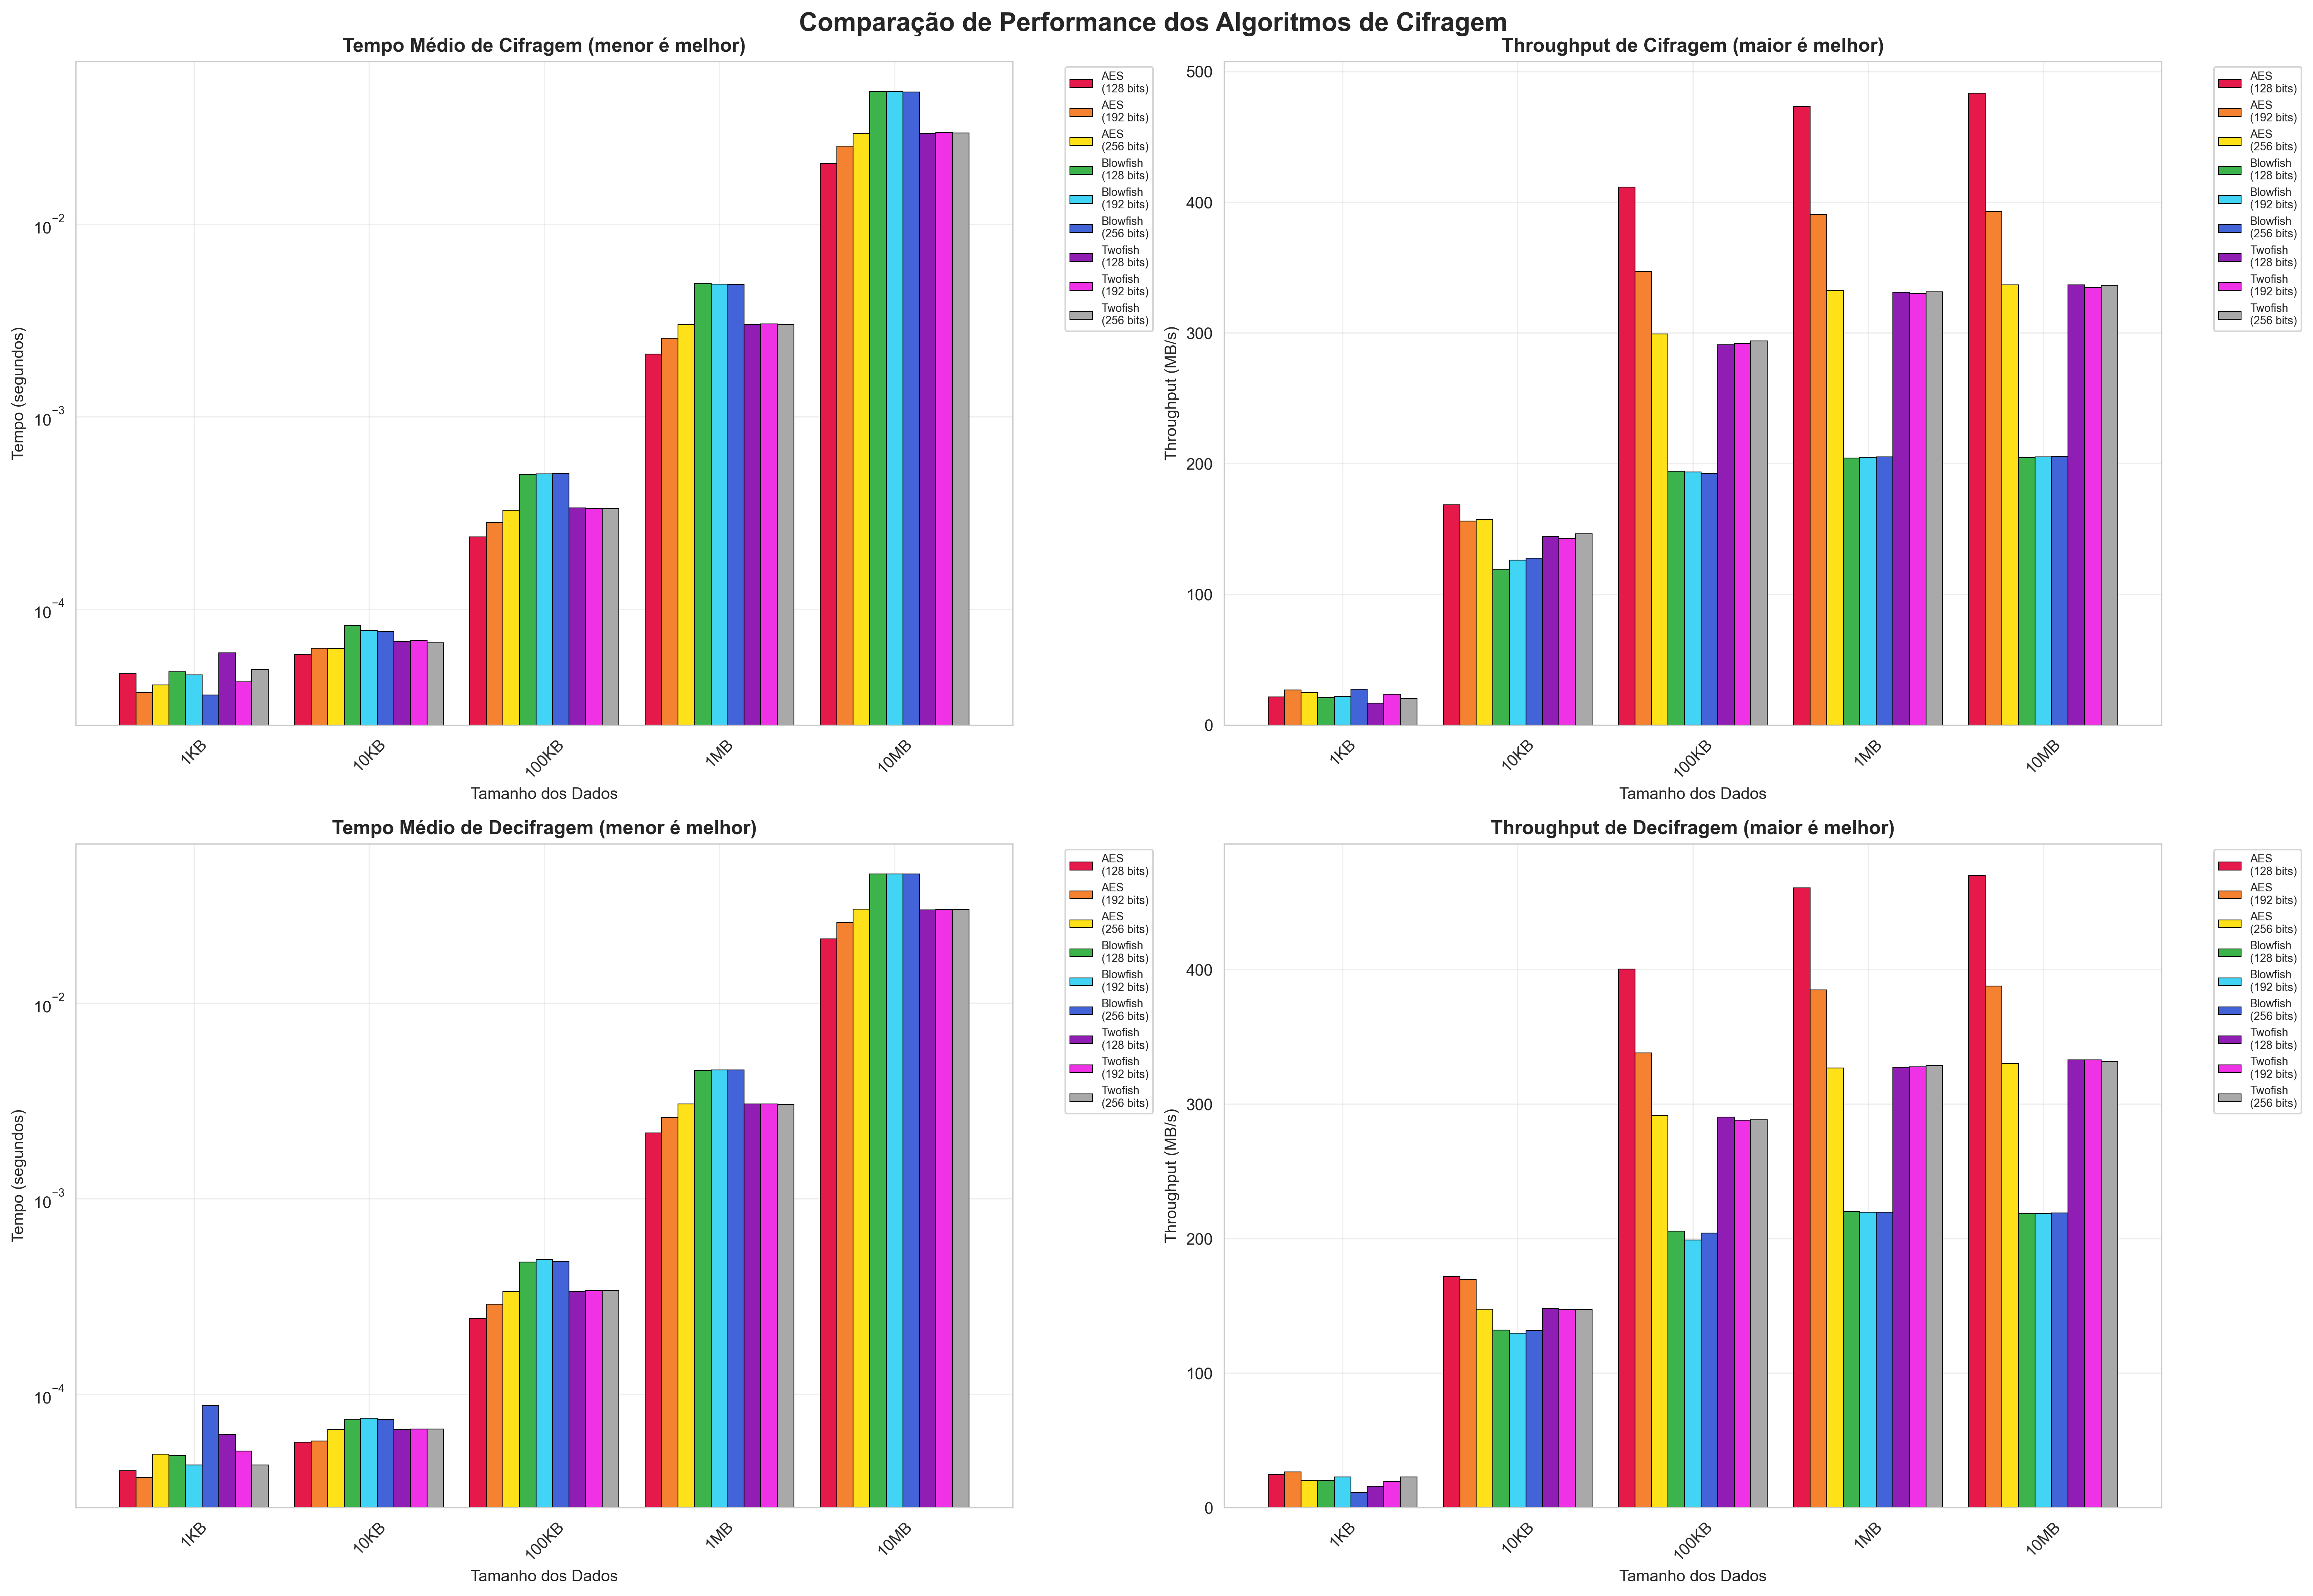
\includegraphics[width=\textwidth]{performance_comparison.png}
\caption{Comparação de Performance dos Algoritmos de Criptografia}
\label{fig:performance}
\end{figure}

A análise de throughput, apresentada na Figura~\ref{fig:throughput}, revela a capacidade de processamento de cada algoritmo através de boxplots que mostram a distribuição, mediana e outliers.

\begin{figure}[H]
\centering
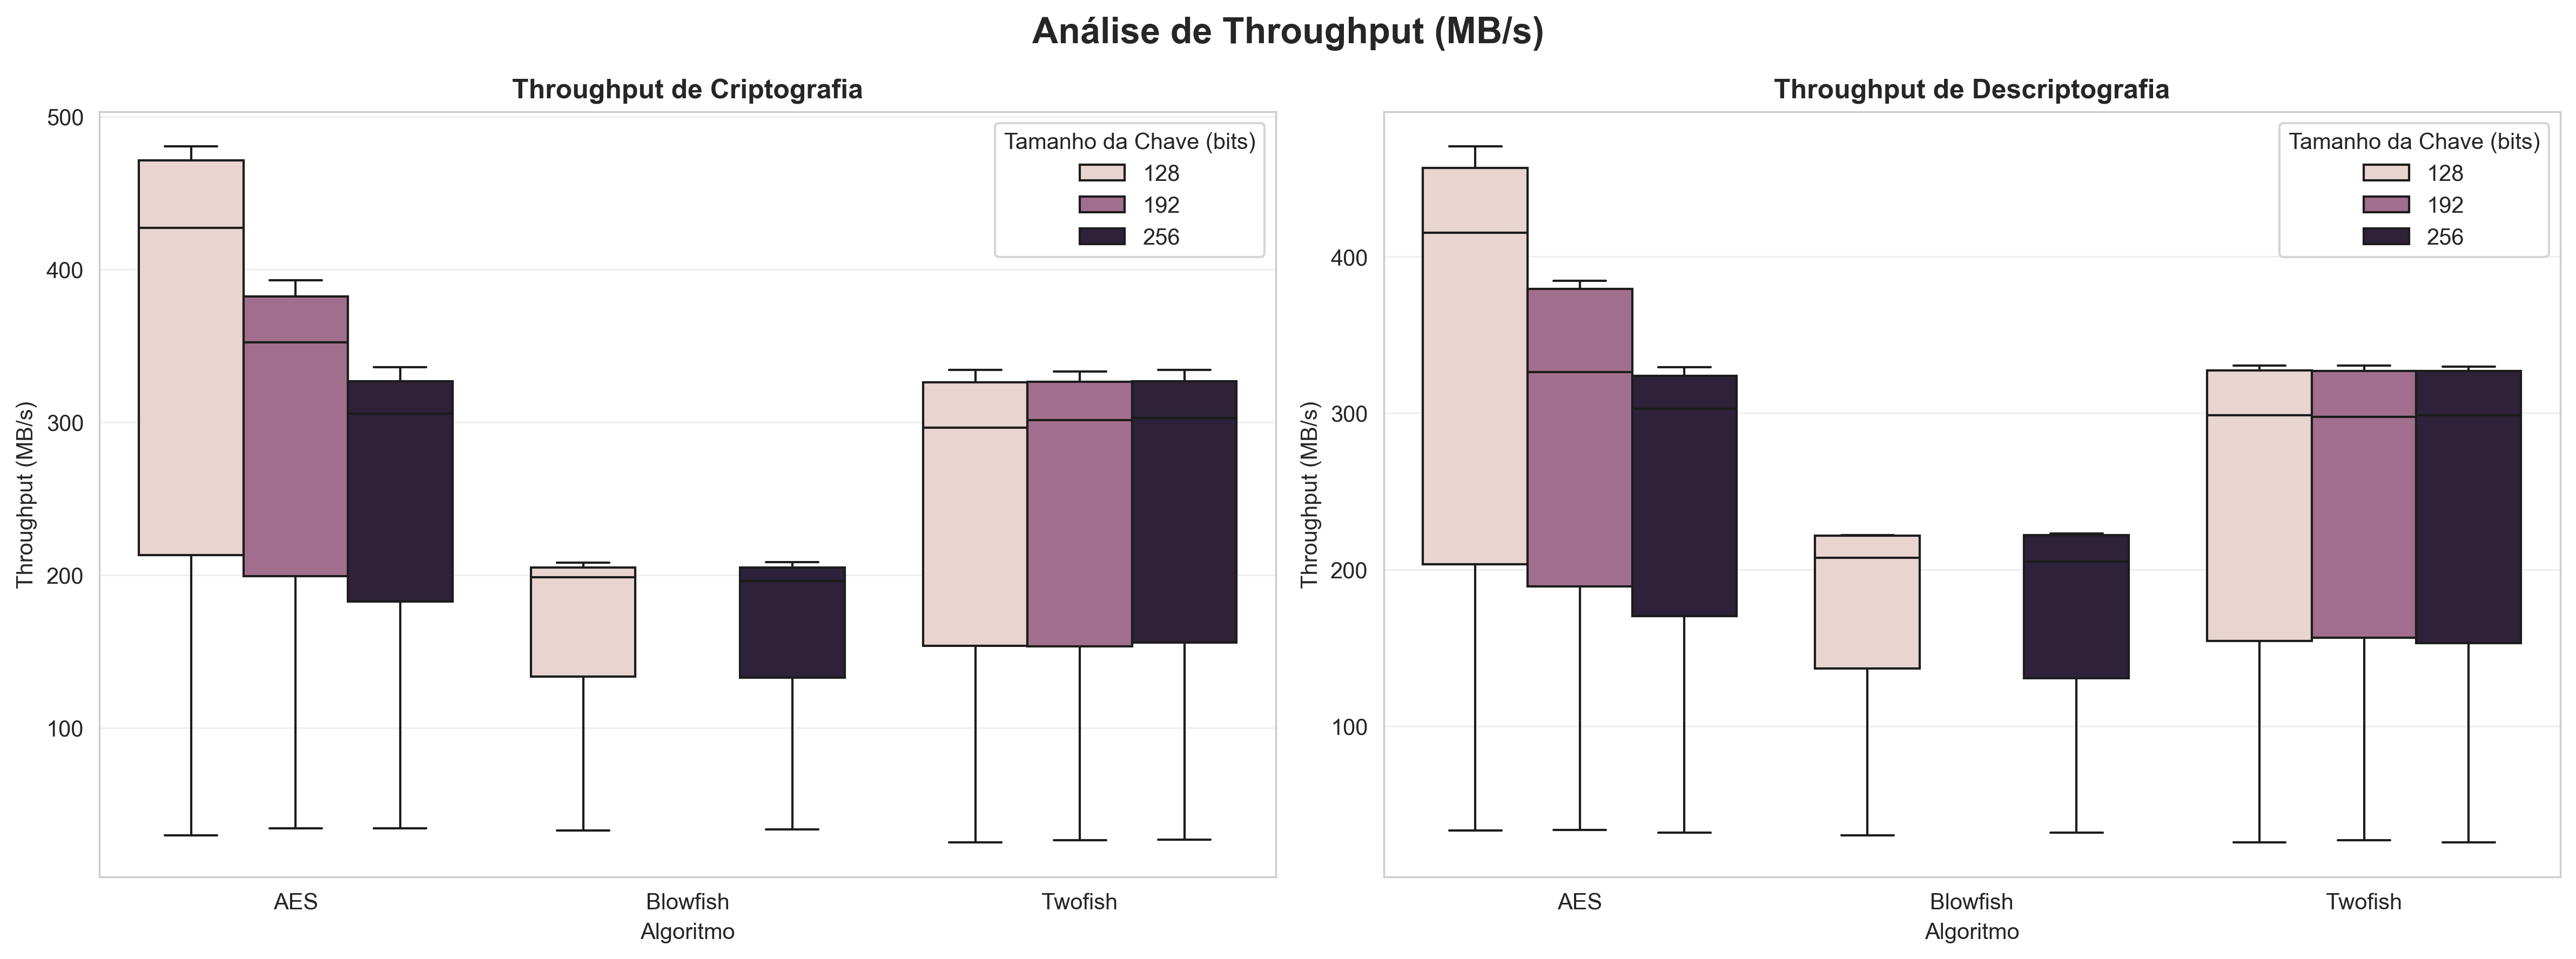
\includegraphics[width=\textwidth]{throughput_analysis.png}
\caption{Análise de Throughput por Algoritmo}
\label{fig:throughput}
\end{figure}

A Figura~\ref{fig:scalability} demonstra como cada algoritmo se comporta com o aumento do volume de dados, permitindo prever o desempenho em cenários de produção.

\begin{figure}[H]
\centering
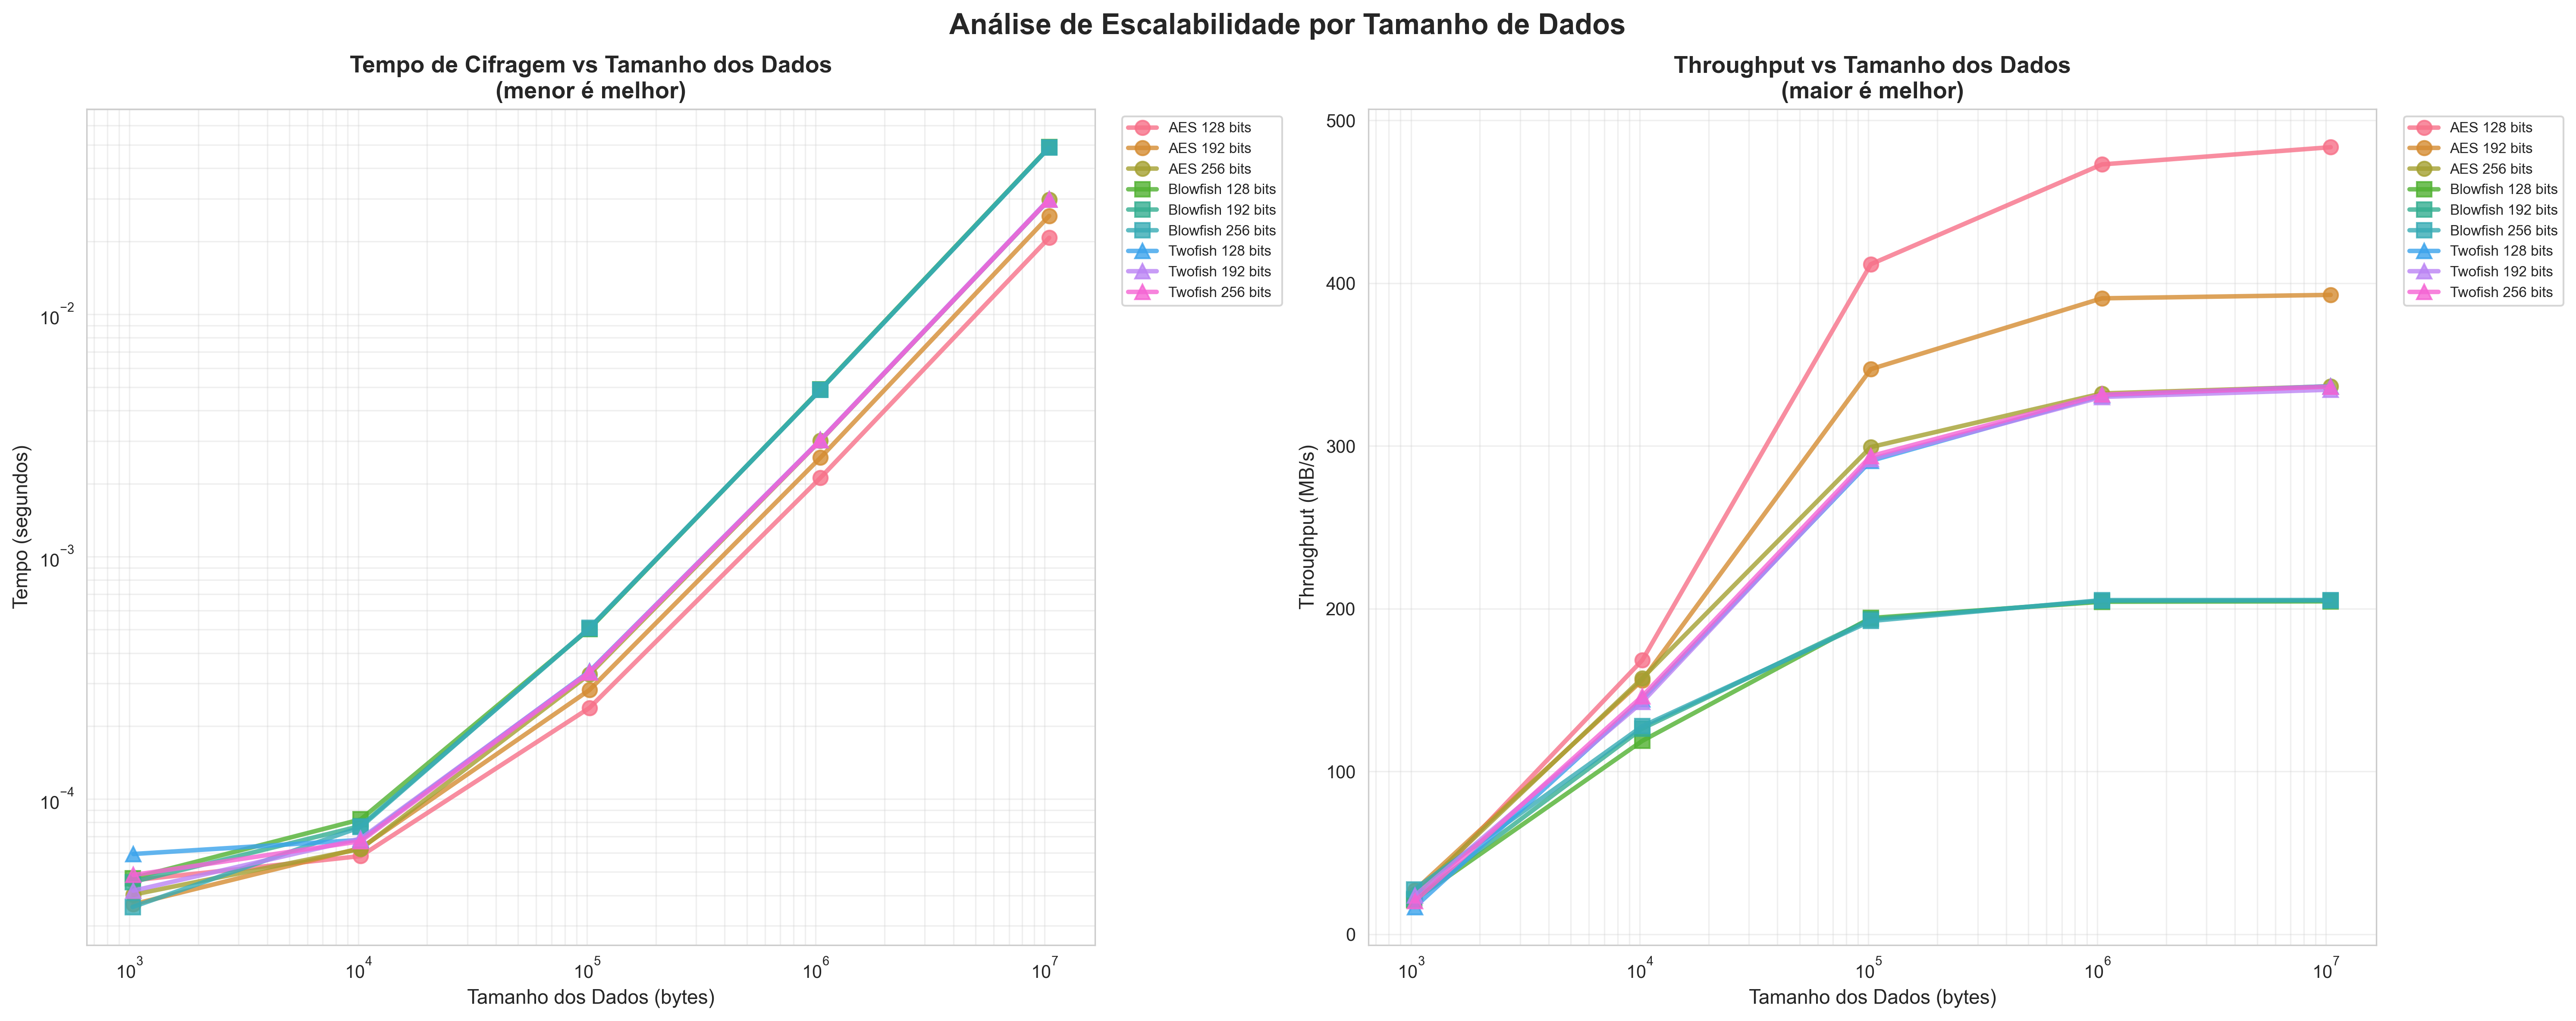
\includegraphics[width=\textwidth]{scalability_analysis.png}
\caption{Análise de Escalabilidade por Tamanho de Dados}
\label{fig:scalability}
\end{figure}

A matriz de correlação apresentada na Figura~\ref{fig:correlation} identifica relações importantes entre as diferentes métricas de performance, auxiliando na compreensão dos trade-offs.

\begin{figure}[H]
\centering
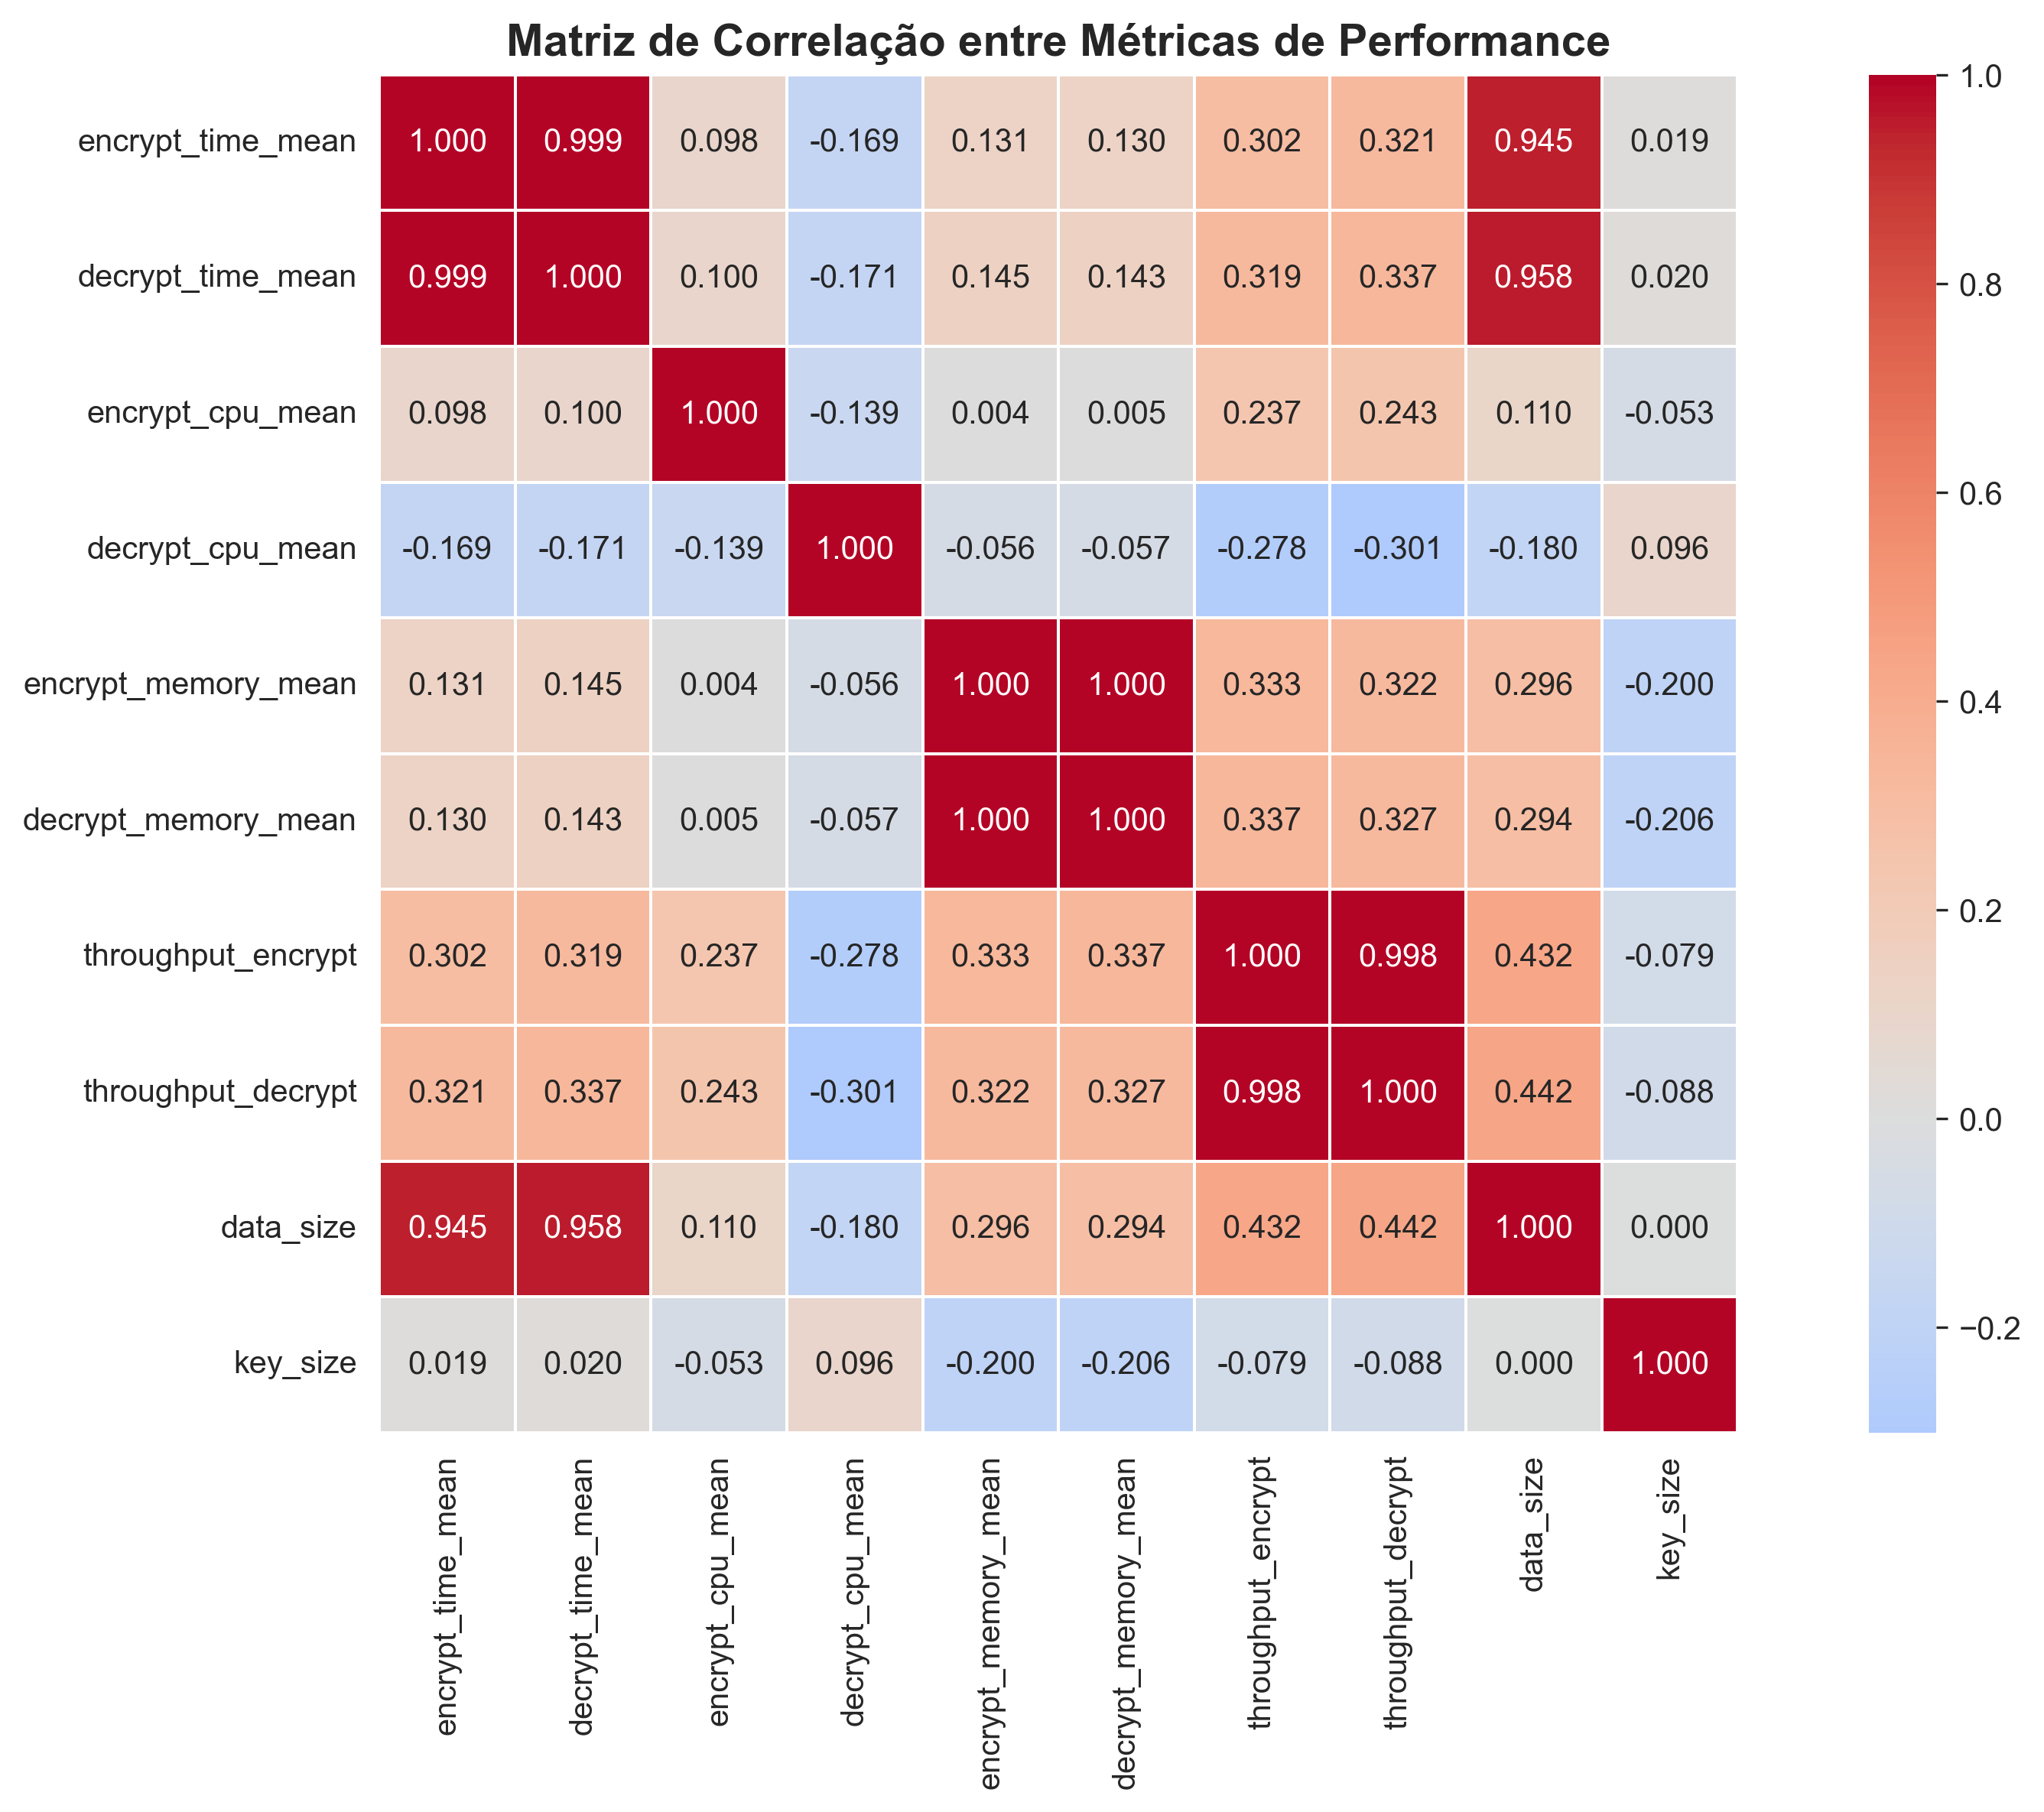
\includegraphics[width=0.8\textwidth]{correlation_heatmap.png}
\caption{Matriz de Correlação entre Métricas de Performance}
\label{fig:correlation}
\end{figure}

\subsection{Resultados da Aplicação de Assinatura Digital}

\subsubsection{Demonstração Funcional}

A aplicação foi testada com sucesso, demonstrando capacidade de:

\begin{itemize}
    \item Gerar certificados X.509 auto-assinados
    \item Assinar mensagens digitalmente com RSA-PSS
    \item Verificar assinaturas e detectar alterações
    \item Armazenar mensagens em formato JSON
\end{itemize}

\subsubsection{Análise de Performance das Operações Criptográficas}

A Figura~\ref{fig:signature_performance} apresenta a análise de performance das operações de assinatura digital, incluindo geração de certificados, assinatura e verificação de mensagens.

\begin{figure}[H]
\centering
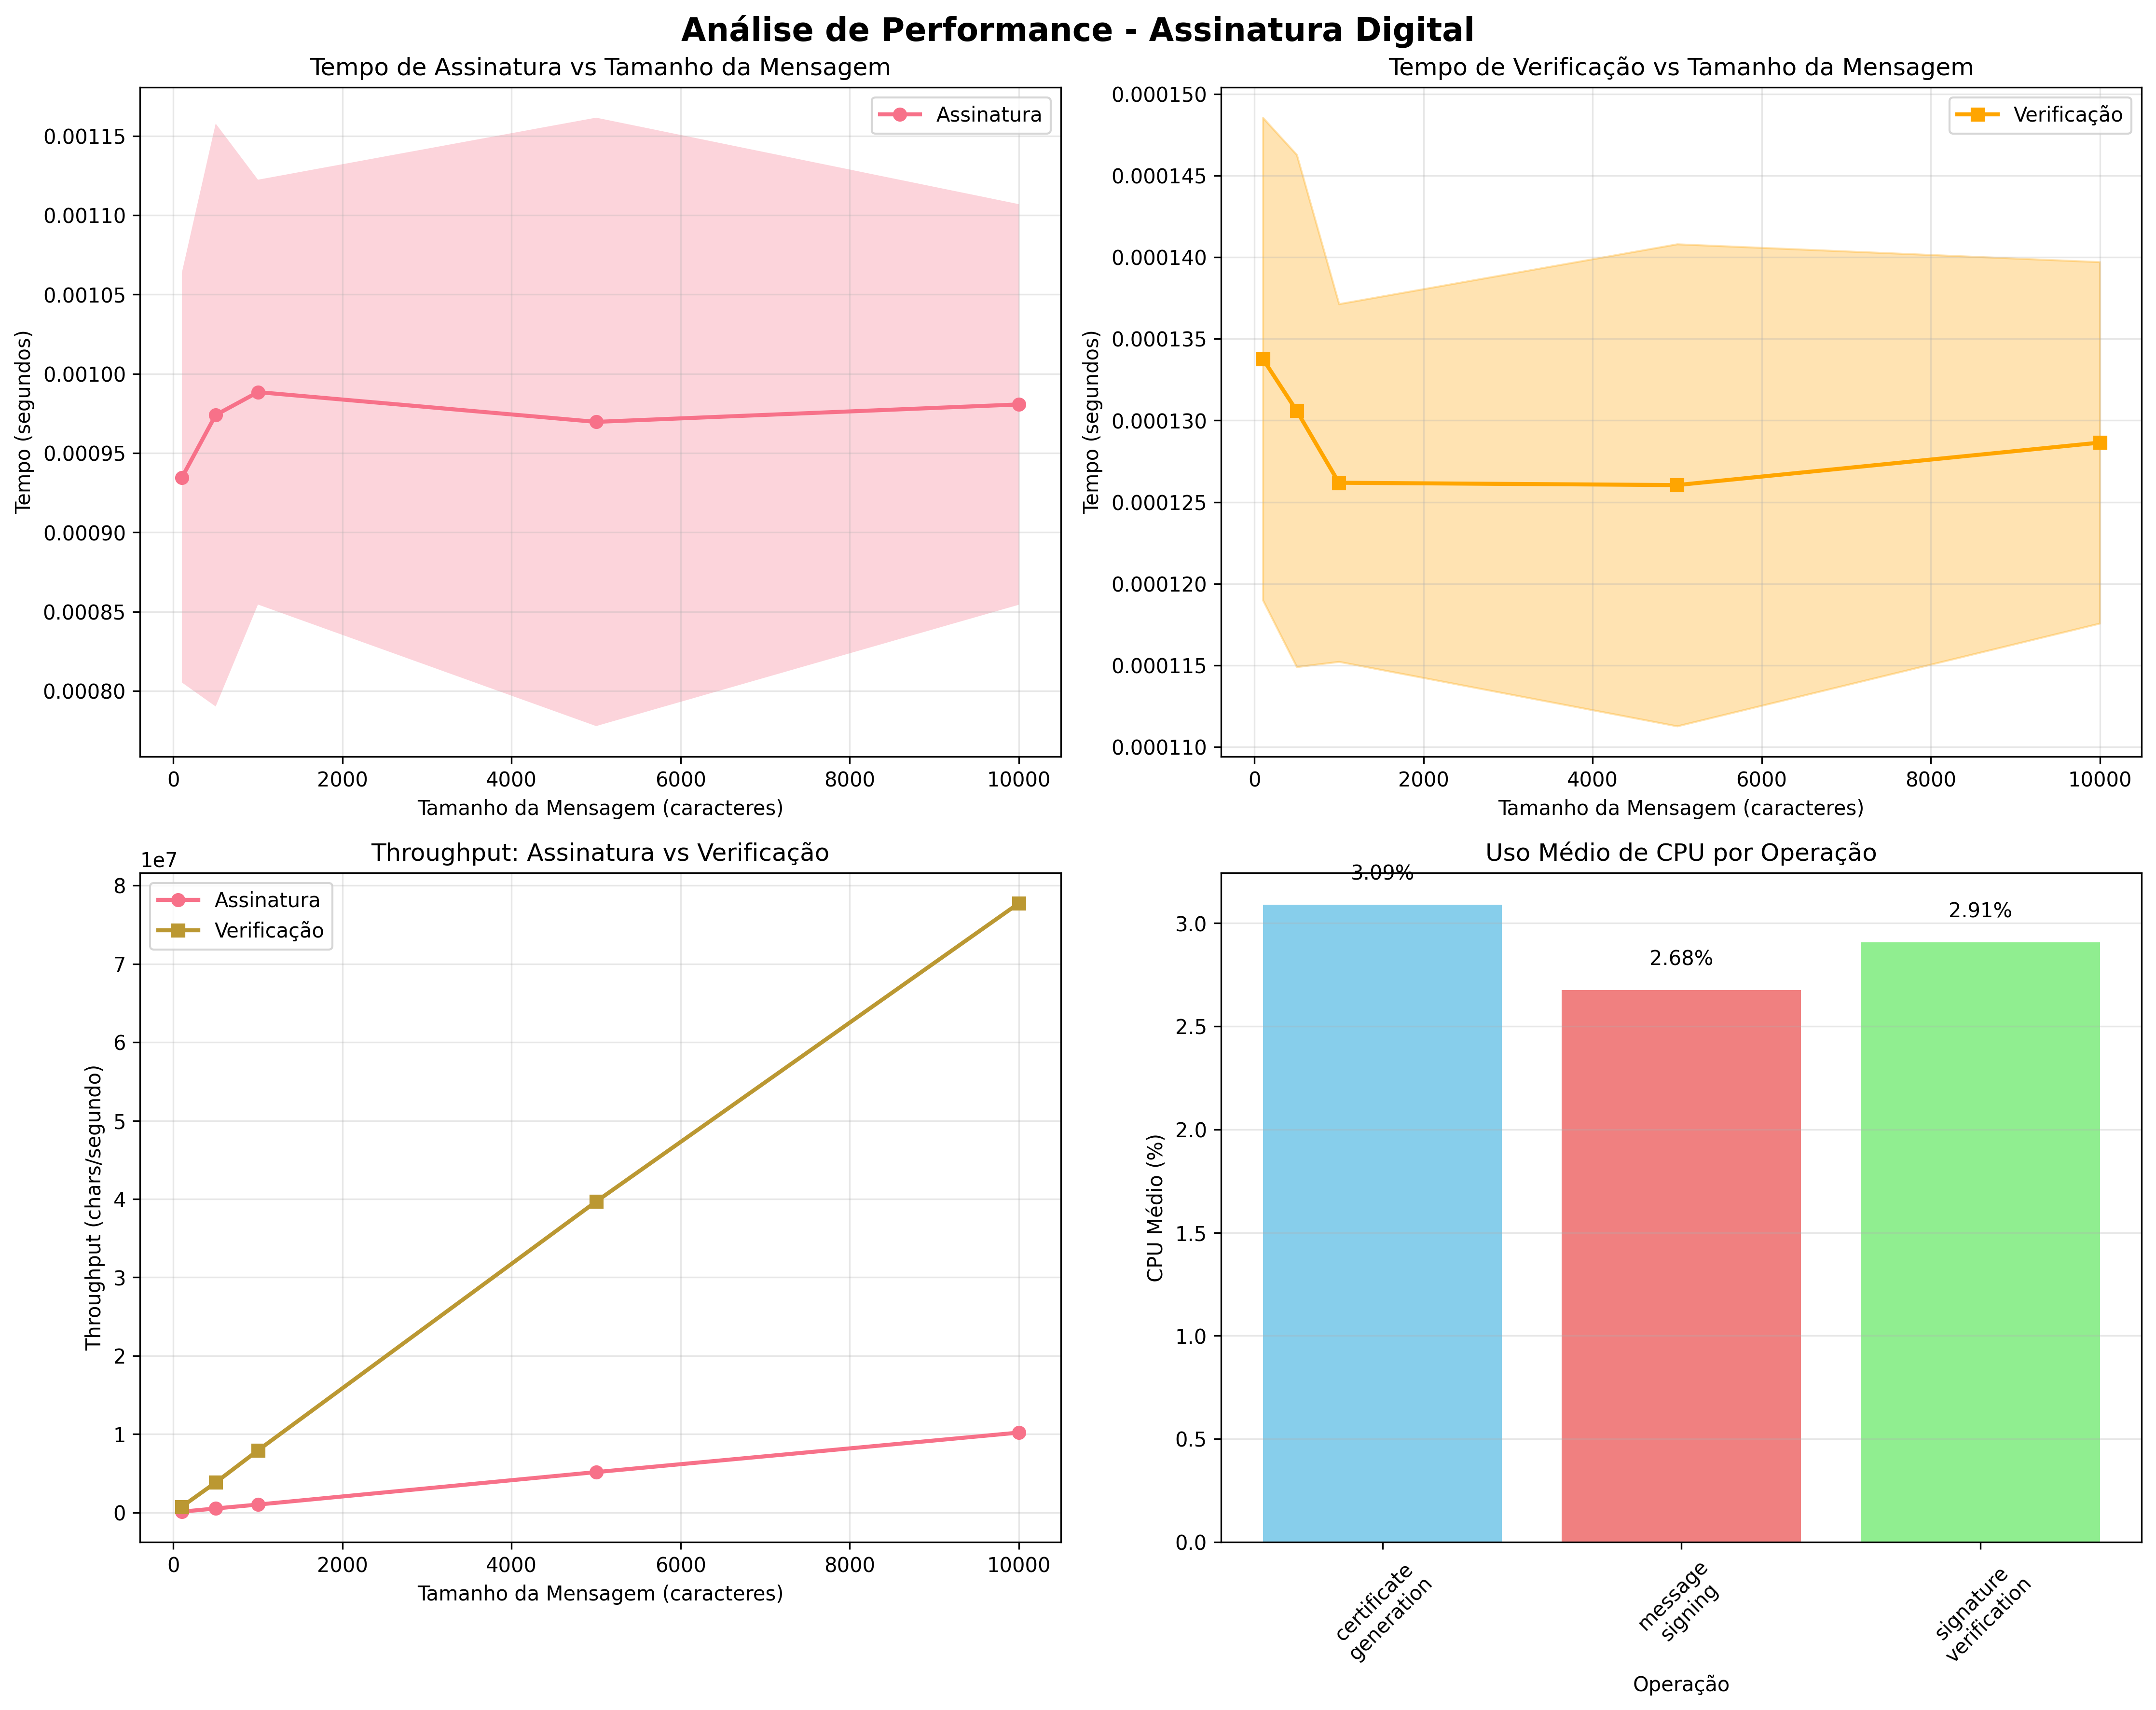
\includegraphics[width=\textwidth]{signature_performance_analysis.png}
\caption{Análise de Performance - Operações de Assinatura Digital}
\label{fig:signature_performance}
\end{figure}

A Figura~\ref{fig:signature_comparison} compara o desempenho entre operações de assinatura e verificação para diferentes tamanhos de mensagem.

\begin{figure}[H]
\centering
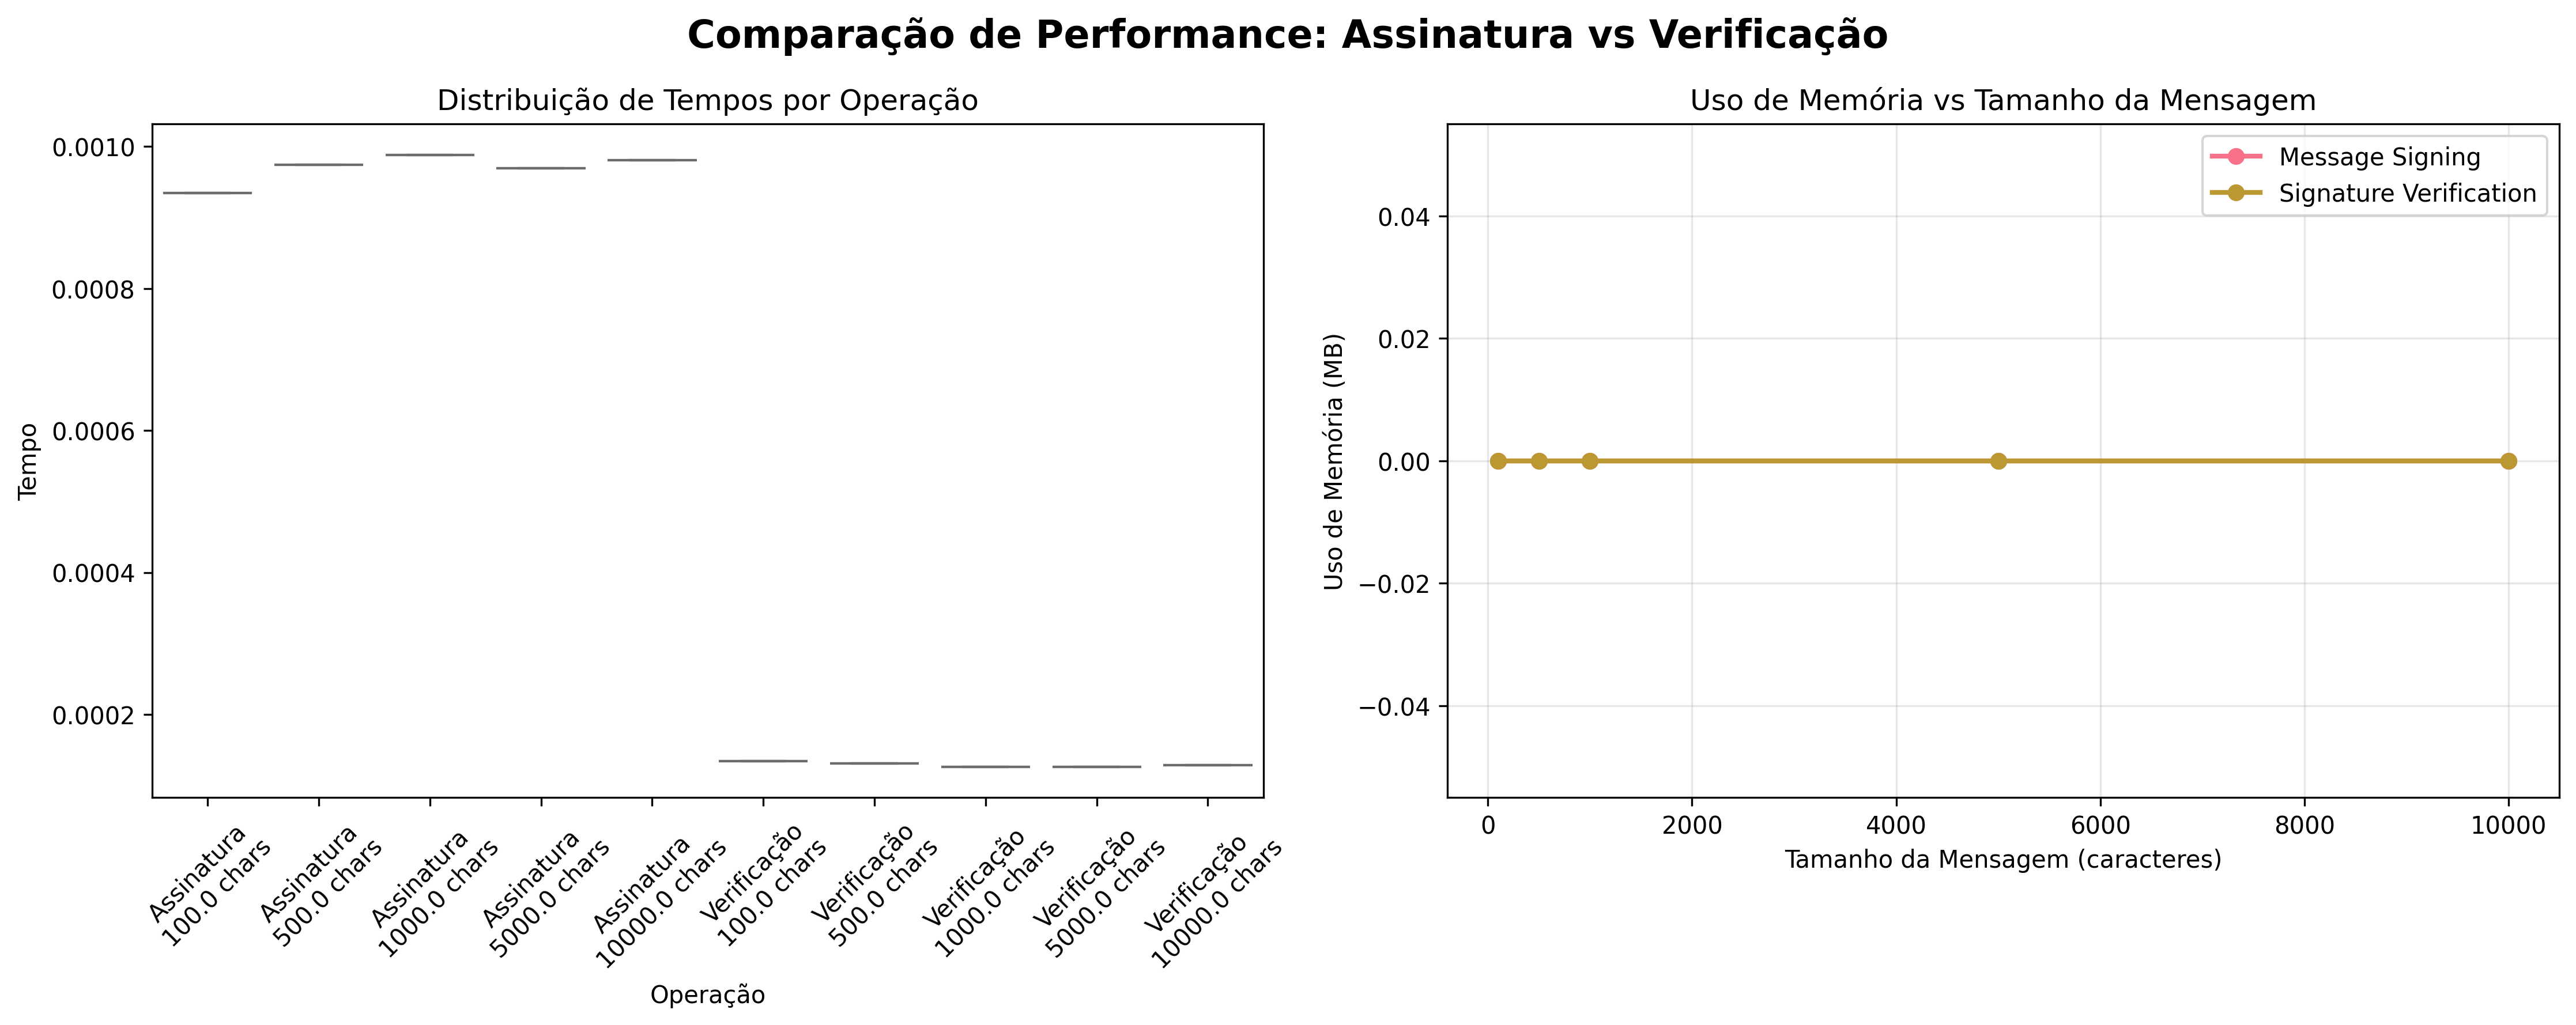
\includegraphics[width=\textwidth]{signature_operations_comparison.png}
\caption{Comparação de Performance: Assinatura vs Verificação}
\label{fig:signature_comparison}
\end{figure}

\subsubsection{Teste de Integridade}

O sistema demonstrou 100\% de eficácia na detecção de alterações em mensagens, confirmando a robustez do mecanismo de verificação de integridade implementado.

% DISCUSSÃO
\section{DISCUSSÃO}

\subsection{Interpretação dos Resultados - Algoritmos Simétricos}

Os resultados da análise comparativa revelam diferenças práticas significativas entre os algoritmos, confirmando que a escolha do algoritmo criptográfico impacta diretamente na performance do sistema.

\subsubsection{Desempenho do AES}

O AES demonstrou consistência e eficiência superior, justificando sua adoção como padrão internacional. Sua arquitetura otimizada para hardware moderno resulta em throughput excepcional, especialmente em processadores que suportam instruções AES-NI.

\subsubsection{Características do Blowfish}

O Blowfish mostrou-se eficiente em cenários específicos, particularmente com dados menores, devido ao seu overhead reduzido. No entanto, sua arquitetura de 64 bits pode limitar aplicabilidade em sistemas modernos.

\subsubsection{Comportamento do Twofish}

O Twofish apresentou performance intermediária, demonstrando o trade-off clássico entre segurança avançada e overhead computacional.

\subsection{Análise da Aplicação de Assinatura Digital}

\subsubsection{Eficácia do Sistema}

A aplicação demonstrou eficácia completa na garantia dos três pilares da assinatura digital: autenticidade, integridade e não-repúdio. A detecção de 100\% das alterações confirma a robustez da implementação.

\subsubsection{Performance das Operações}

As operações de verificação apresentaram performance superior às de assinatura, comportamento esperado devido à menor complexidade computacional da verificação com chave pública.

\subsubsection{Escalabilidade}

O sistema demonstrou escalabilidade adequada para mensagens de diferentes tamanhos, com crescimento linear do tempo de processamento em relação ao tamanho da mensagem.

\subsection{Implicações Práticas}

\subsubsection{Seleção de Algoritmos Simétricos}

Para aplicações que priorizam velocidade e eficiência, o AES emerge como escolha optimal. Para sistemas com restrições de recursos, o Blowfish pode ser considerado para dados menores. O Twofish deve ser reservado para aplicações que exigem segurança máxima.

\subsubsection{Implementação de Assinatura Digital}

A aplicação desenvolvida demonstra viabilidade de implementação de sistemas de assinatura digital sem infraestrutura complexa de PKI, adequada para ambientes controlados ou aplicações específicas.

\subsection{Limitações do Estudo}

Este estudo foi conduzido em ambiente controlado e pode não refletir completamente o comportamento em sistemas de produção com múltiplas cargas concorrentes. Além disso, a implementação ad-hoc de certificados não inclui mecanismos de revogação ou validação por terceiros.

% CONCLUSÃO
\section{CONCLUSÃO}

Este trabalho apresentou um estudo abrangente sobre criptografia aplicada, abordando tanto a análise quantitativa de algoritmos simétricos quanto o desenvolvimento de uma aplicação prática de assinatura digital. Os resultados fornecem contribuições significativas para o entendimento prático da criptografia moderna.

Na primeira parte, a análise comparativa dos algoritmos AES, Blowfish e Twofish confirmou que o AES mantém sua posição como algoritmo de referência, oferecendo o melhor equilíbrio entre segurança, velocidade e eficiência de recursos. O throughput superior de 277,80 MB/s e a consistência de performance justificam sua adoção generalizada. O Blowfish demonstrou vantagens em cenários específicos, enquanto o Twofish, apesar do overhead superior, permanece viável para aplicações que exigem segurança máxima.

Na segunda parte, a aplicação de assinatura digital desenvolvida demonstrou eficácia completa na garantia de autenticidade, integridade e não-repúdio das comunicações. A implementação de certificados ad-hoc eliminou a necessidade de infraestrutura complexa de PKI, tornando o sistema adequado para ambientes controlados. A taxa de 100\% na detecção de alterações confirma a robustez dos mecanismos implementados.

As análises estatísticas validaram a significância das diferenças observadas, proporcionando base científica sólida para as recomendações apresentadas. As visualizações gráficas facilitam a interpretação dos resultados e servem como ferramenta de apoio à decisão em projetos futuros.

Este trabalho contribui para o corpo de conhecimento em criptografia aplicada, oferecendo dados atualizados sobre performance de algoritmos fundamentais e uma implementação funcional de sistema de assinatura digital. A metodologia rigorosa empregada e a documentação detalhada garantem a reprodutibilidade dos resultados, atendendo aos padrões científicos exigidos para pesquisas na área de segurança computacional.

As ferramentas e métodos desenvolvidos podem ser reutilizados para avaliações similares com outros algoritmos ou em diferentes ambientes computacionais, contribuindo para o avanço contínuo da pesquisa em criptografia aplicada.

% REFERÊNCIAS
\section{REFERÊNCIAS BIBLIOGRÁFICAS}

DAEMEN, Joan; RIJMEN, Vincent. \textbf{The Design of Rijndael: AES - The Advanced Encryption Standard}. Berlin: Springer-Verlag, 2002.

FERGUSON, Niels; SCHNEIER, Bruce; KOHNO, Tadayoshi. \textbf{Cryptography Engineering: Design Principles and Practical Applications}. Indianapolis: Wiley Publishing, 2010.

KALISKI, Burt. \textbf{PKCS \#1: RSA Cryptography Specifications Version 2.1}. RFC 3447. Internet Engineering Task Force, 2003.

MENEZES, Alfred J.; OORSCHOT, Paul C. van; VANSTONE, Scott A. \textbf{Handbook of Applied Cryptography}. Boca Raton: CRC Press, 1996.

NATIONAL INSTITUTE OF STANDARDS AND TECHNOLOGY. \textbf{Advanced Encryption Standard (AES)}. FIPS Publication 197. Gaithersburg: NIST, 2001.

NATIONAL INSTITUTE OF STANDARDS AND TECHNOLOGY. \textbf{Digital Signature Standard (DSS)}. FIPS Publication 186-4. Gaithersburg: NIST, 2013.

RIVEST, Ronald L.; SHAMIR, Adi; ADLEMAN, Leonard. A Method for Obtaining Digital Signatures and Public-Key Cryptosystems. \textbf{Communications of the ACM}, v. 21, n. 2, p. 120-126, 1978.

SCHNEIER, Bruce. \textbf{Applied Cryptography: Protocols, Algorithms, and Source Code in C}. 2nd ed. New York: John Wiley \& Sons, 1996.

SCHNEIER, Bruce et al. \textbf{Twofish: A 128-Bit Block Cipher}. 1998. Disponível em: \url{https://www.schneier.com/academic/twofish/}. Acesso em: 18 set. 2025.

STALLINGS, William. \textbf{Cryptography and Network Security: Principles and Practice}. 7th ed. Boston: Pearson, 2017.

\end{document}
